\documentclass[11pt,a4paper]{article}
\usepackage[margin=1in]{geometry}
\usepackage[T1]{fontenc}
\usepackage[utf8]{inputenc}
\usepackage{lmodern}
\usepackage{hyperref}
\usepackage{enumitem}
\usepackage{xurl}
\usepackage{tikz}
\usepackage{float}
\usetikzlibrary{arrows.meta, positioning, shapes.geometric}
\hypersetup{colorlinks=true,linkcolor=blue,urlcolor=blue}
\newcommand{\codepath}[1]{\path{#1}}
\tikzset{box/.style={rectangle,draw,rounded corners,align=center,inner sep=3pt,minimum width=36mm},line/.style={-Latex}}

\title{Phase-2 Deliverable: Golden Micro-kernel Traces}
\author{SIT Engine Architecture}
\date{\today}

\begin{document}
\maketitle

\section{Technical Description}
Golden micro-kernel traces are deterministic workload executions used as anchor datasets for simulator comparison and regression checks. They establish repeatable input signals for SIT behavior validation.

\section{Implementation Fulfillment}
Trace generation and indexing are implemented through:
\begin{itemize}[leftmargin=*]
  \item workload execution/orchestration: \codepath{Phase-2/riscvbench.py},
  \item spike golden pipeline: \codepath{Phase-2/tests/run_spike_golden_pipeline.py},
  \item qemu golden pipeline: \codepath{Phase-2/tests/run_qemu_golden_pipeline.py},
  \item dataset baseline manifest: \codepath{Phase-2/datasets/manifest.json}.
\end{itemize}
Produced artifacts include per-run \codepath{trace.csv}, pipeline \codepath{trace\_index.csv}, and generated manifests.

\section{Design \& Architecture}
Golden trace flow is matrix-driven (workload, size, flag mode). Each case runs target-specific execution, then adapters normalize output and register trace metadata. This provides a deterministic replay surface for invariant and monotonic checks.

Current gap to close for done-when: maintain pinned golden bundles for all intended simulators with explicit versioned directories and review policy.

\subsection*{Function Flowchart}
\begin{figure}[H]
\centering
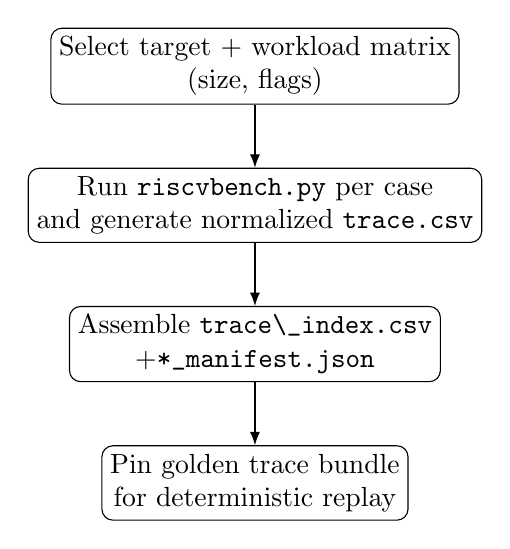
\begin{tikzpicture}[node distance=8mm and 12mm]
\node[box] (a) {Select target + workload matrix\\(size, flags)};
\node[box, below=of a] (b) {Run \codepath{riscvbench.py} per case\\and generate normalized \codepath{trace.csv}};
\node[box, below=of b] (c) {Assemble \codepath{trace\_index.csv}\\+\codepath{*_manifest.json}};
\node[box, below=of c] (d) {Pin golden trace bundle\\for deterministic replay};
\draw[line] (a) -- (b);
\draw[line] (b) -- (c);
\draw[line] (c) -- (d);
\end{tikzpicture}
\caption{Golden Micro-kernel Trace Flow}
\end{figure}

\end{document}
